\documentclass[conference]{IEEEtran}
% Packages
%\pdfobjcompresslevel=0
\usepackage{titlesec}
\usepackage{graphicx}
\usepackage{lipsum} % For dummy text, you can remove this
\usepackage[style=numeric, backend=biber]{biblatex} % Import the package for reading .bib files
\addbibresource{Communication.bib} % Add the .bib file
\usepackage{algorithm}
\usepackage{algpseudocode}
\usepackage{booktabs}

% Title page
\title{Dissertation Title}
\author{Luis Yallico Ylquimiche}
\date{\today}

\begin{document}

% Title page
\maketitle

% Abstract
\begin{abstract}
LOREM IPSUM
\end{abstract}


\section{Introduction}

Swarm engineers draw inspiration from social biological systems such as ants or bees to build decentralised robot collectives that are inherently robust to failure, flexible across tasks and scalable in number \cite{dias_swarm_2021}. In swarm systems, collective intelligence emerges when individual robots trade packets of information among neighbouring robots. Classic ant-colony-optimisation (ACO) work in the early 2000s has already proven that an indirect information exchange "virtual-pheromones" can lead to agents collectively discovering optimal routing behaviours \cite{dorigo_ant_2000}. Highlighting the importance of communication design in swarms and the effect it can have over their behaviour.\\

Moreover, communication remains the least measured layer of swarm robotics. A recent survey by \cite{an_multi-robot_2023} found that the majority of swarm studies focus on coordination and task allocation, with relatively little focus on information exchange. Notwithstanding this, it was reported that bandwidth, latency and energy usage are now the main blockers to real-world swarm deployments. Parallel conclusions have been made by \cite{ding_advancements_2023}, whom suggests that researchers are challenged by the increasing data volume transmitted among swarm peers. As the number of agents grows so does the throughput of the network, which can exceed a single agent's processing capabilities as these tend to be hardware limited.\\

Beyond the swarm's capacity, the architecture of the communication also matters. In many direct communication schemes, broadcasting is a common mode of data transmission across various swarm deployments \cite{an_multi-robot_2023}. For example,\cite{perrin_decentralised_2012} demonstrated that peer-to-peer broadcasts allowed swarms to map unknown environments in disaster zones. However, this type of data flooding is known to scale poorly \cite{an_multi-robot_2023}, this due to increasing Wi-Fi collision rates once swarms grow past a few dozen peers.\\ 

Furthermore, embodied evolution of swarm controllers heavily relies on communication to tune the controller. Some recent studies explain that less communication can sometimes enhance swarm performance, as trimming neighbourhood size helps populations forget outdated beliefs and re-adapt faster \cite{hiraga_when_2023}\cite{ding_advancements_2023}. Most of these studies were performed in simulation, hence the need for empirical data on how swarm density, rate of data transfer and packet content affects evolution performance. With this in mind, it is possible to think of communication as a dynamic resource that can be manipulated by the swarm to achieve its goals. The ways in which this resource is allocated can have a significant impact on the behaviour of the swarm.\\

This study addresses some of these gaps by exploring different communication protocols in a swarm system. To do this we deploy collective built on the low-cost ESP32 microcontrollers, that to our knowledge have not yet been profiled in swarm literature. Focusing on direct peer to peer ESP-NOW data transfer, we log key performance indicators such as latency, error rates, core usage and evolution metrics while systematically varying density, locomotion, topology awareness, imposed message budgets and stochastic transmission. Our goals are to (i) extend existing communication taxonomies to the ESP32/IoT hardware class, (ii) provide concrete data for the integration challenges flagged by literature, and (iii) translate abstract guidance on swarm communication into tangible design rules.

\section{Related Work}

%add This is based on the Island model [ref], where different subpopulations (islands) evolve in parallel and occasionally exchange individuals (migration) with other islands, thus enabling the swarm to converge to a solution. 

%We utilized the built-in WiFi capabilities of the ESP32 with the ESPNOW communication protocol, which supports multiple unicast connections. While ESPNOW can theoretically handle around 20 devices simultaneously, practical limits are dictated by environmental factors. Additionally, ESPNOW enables multicast data transmission to multiple devices on the same channel, which can be used to pair devices or send messages to multiple swarm members. The protocol operates at a default bitrate of approximately 1 Mbps, although a portion of this bandwidth is consumed by necessary overhead, such as the MAC header. 

%For expanding a swarm dynamically, cryptographic keys might be needed to securely onboard new members, this however is out of scope of the current study.

%one way communication

\section{Experimental Setting}

In this study, a global optimisation problem known as the Rastrigin function Eq. \ref{eq:rastrigin} is used to benchmark the communication performance in a swarm with up to 13 agents. This task was chosen to emulate evolutionary controller optimisation, while no controller was actually evolved the concept of robots sending and receiving genomes from their peers remained the same.\\ 

The environment for the experiments was a rectangular arena without obstacles (Figure \ref{fig:arena}), where the initial positions, orientations and number of the robots was determined by the type of experiment being conducted (Section X). All of the experiments were conducted in the same room environment within the department of Engineering Mathematics at the University of Bristol.

\begin{figure}[h]
    \centering
    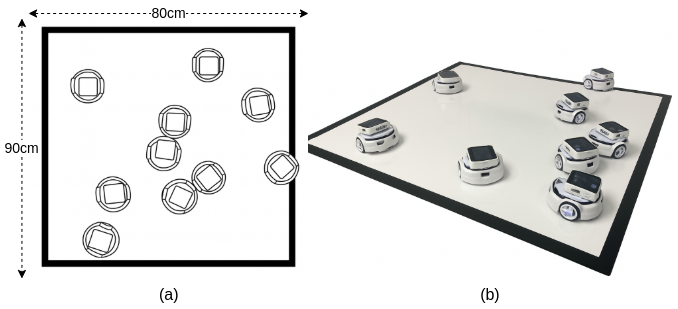
\includegraphics[width=0.49\textwidth]{arena.png}
    \caption{Robot Arena: (a) dimensions and (b) example of locomotion experiment with 8 robots.}
    \label{fig:arena}
\end{figure}


\subsection{Rastrigin Function}

The Rastrigin function is defined as follows:

\begin{equation}\label{eq:rastrigin}
f_R(\mathbf{x}) = 10n + \sum_{i=1}^{n} \left(x_i^2 - 10\cos(2\pi x_i)\right)
\end{equation}

where $n$ is the number of dimensions, in this case the number of genes. Whereas, $x$ is the individual genome being evaluated. The function has a global minimum at \( f_R(\mathbf{x}) = 0 \) when $x = [0, 0, ..., 0]$ for all dimensions \cite{rucinski_impact_2010}. For the purpose of this study we used $n = 10$ and a solution bounded at $-5.12<=x_i<=5.12$.

\subsection{Robot Platform}\label{sec:robot_platform}
\begin{figure}[h]
    \centering
    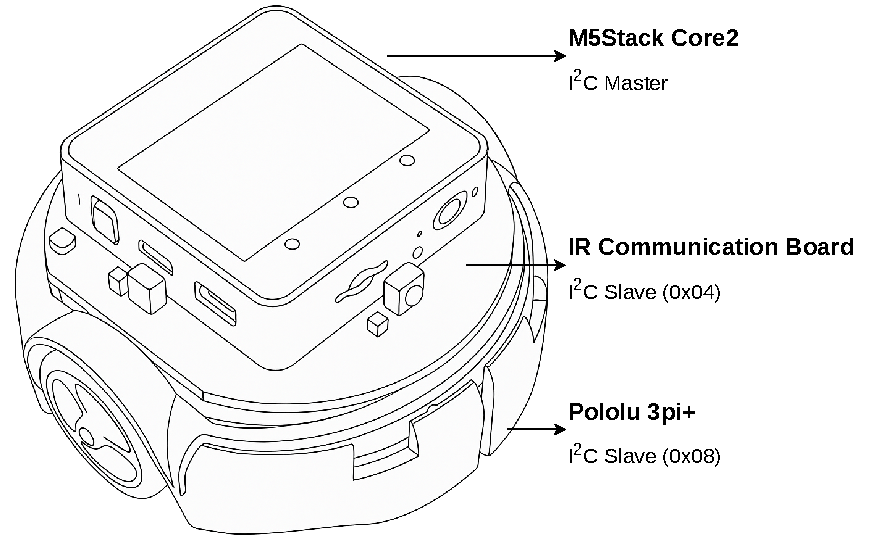
\includegraphics[width=0.45\textwidth]{B2.pdf}
    \caption{The Swarm-B2 platform: M5Stack Core2, IR Communication board, and Pololu 3Pi+}
    \label{fig:B2}
\end{figure}

Table~\ref{tab:B2-hardware} summarises the core hardware components of the Swarm-B2 platform used in this study REF. The ESP32 microcontroller acts as the I\textsuperscript{2}C master, coordinating an communication board and a Pololu~3Pi+ driver base over a 100kHz bus. Although the IR board can transmit/receive 32-byte frames, the experiments reported here have disabled this feature. The board therefore behaves as a I²C bridge between the M5 master and the Pololu 3Pi+ slave. This guarantees that the communication results discussed in Section REF stem only from the ESP-NOW protocol.\\

\begin{table}[h]
  \centering
  \caption{Swarm-B2 hardware stack}
  \label{tab:B2-hardware}
  \begin{tabular}{p{0.20\linewidth} p{0.22\linewidth} p{0.40\linewidth}}
    \toprule
    Component & Interface(s) & Function \\
    \midrule
    M5Stack Core2 (240 MHz) & I\textsuperscript{2}C master and SPI & Solve Rastrigin, ESP-NOW communication, data logging to SD and user interface \\
    IR board (16 MHz) & I\textsuperscript{2}C slave (0x04) & Bus hub, optional IR feature \\
    Pololu 3Pi+ (16 MHz) & I\textsuperscript{2}C slave (0x08) & Locomotion, bumper and line following sensors \\

    \bottomrule
  \end{tabular}
\end{table}

The ESP32 was used as the master device is because of the SD card support which is discussed in Section X and because of its larger flash memory. Furthermore, with 8MB PSRAM and its integrated Wi-Fi support, this microcontroller was capable of running dual-core FreeRTOS tasks (Section X comms on core 0, experiment on core 1) without starving other peripherals. In contrast, the Pololu's board was not able meet the memory bandwidth required for concurrent SD card writes. Making the ESP32 the master also avoided multi master arbitration and simplified bus timing.

\subsubsection{Locomotion}

The Pololu 3Pi+ is equipped with a line following sensor array and two bump sensors, which can be used to detect obstacles and detect the arena edges. We leverage this components to execute a \emph{Brownian-motion} gait that continuously drives the robot through the arena while producing an unbiased spatial trace. Using Brownian motion avoids any preferential trajectory that could skew communication statistics, and is able to keep all agents in motion throughout the run.\\

The gait code exposes the Pololu slave to the ESP32 master node, this interface lets the ESP32 act as a passenger with override, that can set wheel-speed scaling factors or raise \texttt{START}/\texttt{STOP} flags without touching the low-level control loop.  In effect, the Pololu driver handles continuous motion, while the ESP32 decides when to go for each experimental condition (Section X).

\subsubsection{Data Capture}
We implemented local data logging mechanism (Section X) on the ESP32 with a 16GB SD card peripheral. The shared SPI bus (with the LCD) was set at a frequency of 20MHz and configured to use the FAT32 file system for storage. This approach was chosen to emulate a realistic swarm system capable of operating remotely without relying on a stable Wi-Fi connection to a central server. The additional benefit of the local data capture is that it minimizes data transmission loss during the experimental runs.\\

Upon completing each run, the swarm members switch to a data upload mode and connect to the Wi-Fi, where the locally collected data is securely transmitted to an AWS S3 bucket using HTTPS. This might seem counter intuitive to our original objective, but it was planned to be this way as otherwise we would have to manually read each individual SD card to collect the data, which would be time consuming and error prone. Furthermore, we expect that in a real-world scenarios, the swarm would be deployed in a remote location where manual data collection would be impossible.\\

Data logs are saved in the root directory of the SD card in a \.json format. Our system is designed to automatically generate new files upon reaching a specified size limit of 1MB, this enables efficient memory management and preventing heap memory overflow during log file writes.

\subsubsection{User Interface}

\begin{figure}[h]
    \centering
    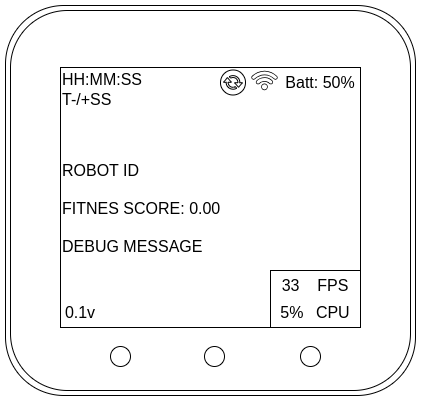
\includegraphics[width=0.35\textwidth]{UI.png}
    \caption{M5 user interface showing the current fitness score and device information.}
    \label{fig:UI}
\end{figure}

Figure \ref{fig:UI} shows the on-board user interface (UI) each Swarm-B2 agent displays during trials. A real-time clock (RTC) seeds a unique \emph{experiment\_id}, just below a $T\pm SS$ counter tells the operator how long until the next minute aligned run. Note that between peers there is an RTC's $\pm1$ drift, this is discussed in Section X. Status lines on the display list the robot's ID (last four hex digits of the MAC address), the live fitness score, and a single debug message. The bottom-left tag logs which software build is running on the device. Two icons round out diagnostics, the Wi-Fi symbol flashes during S3 log upload, and the circular arrow signals an over-the-air update.

\section{Implementation}

In this section we describe the software design and implementation of the swarm firmware. Note that we chose the Espressif IoT development framework (ESP-IDF) for this deployment. This choice was made as first and foremost, it is the official development framework maintained for the ESP32. Unlike the Arduino IDE, which acts as an abstraction layer over ESP-IDF, it provides native and direct access to low level hardware, resulting in greater flexibility for the ESP-NOW communication protocol (discussed Section X).\\

Secondly, ESP-IDF enabled the direct use of FreeRTOS, used for concurrent task creation and multi core processing over the dual-core architecture of the ESP32. This was particularly beneficial in this study as it permits isolating communication specific tasks to an individual core.\\ 

Finally, ESP-IDF is recognized as the industry standard development environment for ESP32 IoT applications. It supports advanced features such as Over-the-Air (OTA) firmware updates (Section \ref{sec:ota}), unit testing and bespoke debugging capabilities. \cite{esp-boards_esp-idf_nodate}.

\subsection{Software Development Environment}\label{sec:SDK}

During the software development and experiment cycles, the Continuous Integration and Continuous Deployment (CI/CD) framework was used, depicted in Figure \ref{fig:cicd-architecture}. This framework enabled automated OTA updates to all agents, eliminating the need for manual flashing of each individual node between experimental runs.\\

The CI/CD integration proved especially valuable when expanding the scope of experiments, where consistent updates across multiple agents were necessary. It also facilitated easier rollbacks in the event of unexpected bugs, thereby increasing the reliability of the experimental results. The automated build pipeline in GitHub ensured that only validated firmware versions were propagated to the swarm, catching any environment discrepancies early in the process.\\

\begin{figure}[h]
    \centering
    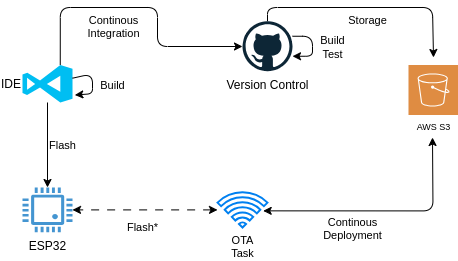
\includegraphics[width=0.45\textwidth]{architecture.png}
    \caption{CI/CD Architecture: Local development, GitHub repository, AWS S3 storage, and OTA updates.}
    \label{fig:cicd-architecture}
\end{figure}

Our software development framework for the swarm is as follows:

\begin{enumerate}
    \item \textbf{Local environment development}: The ESP32 application development takes place locally using VSCode, our local environment uses version 5.1.4 of ESP-IDF and Python 3.11 to build and flash the code in-situ. This self contained development environment allows for testing new features and updates without affecting previous versions of the application running on the swarm.\\
    \item \textbf{Version control}: Once we finish working on a feature, we push the codebase to a public repository on GitHub: \url{https://github.com/yallico/robotics_dissertation}, this allows for version control and triggers a custom build and test process. The ESP32 project is then compiled and generates the binary file used for OTA. This process ensures that the codebase is always in a working state and ready for deployment.\\
    \item \textbf{Cloud storage}: The OTA binary file is uploaded to an AWS S3 public bucket. S3 serves as a reliable and low cost storage solution for the OTA updates. Note that encryption is out of scope for this OTA implementation, yet we acknowledge that this is a non-trivial task for swarms.\\
    \item \textbf{OTA process}: All agents, run a task that is triggered upon initialisation which compares its current flash version against the latest version available in S3. If the S3 version diverges from the local version, the ESP32 downloads the latest .bin file and installs it locally.

\end{enumerate}

\subsubsection{OTA}\label{sec:ota}

Our system uses cloud infrastructure to distribute encrypted update files, this meant that during initialisation we exposed the swarm to the internet via Wi-Fi. It maybe counter-intuitive to rely on a central server to manage swarm firmware updates, however in the future it might be possible to use decentralized storage solutions to avoid having to connect to the internet.\\

\begin{table}[h]
  \centering
  \caption{System Partition Table}
  \begin{tabular}{l l l p{4.3cm}}
  \toprule
  \textbf{Name} & \textbf{Type} & \textbf{Size} & \textbf{Description} \\
  \midrule
  \texttt{nvs} & data & 16KB & Non-volatile storage \\
  \texttt{otadata} & data & 8KB & OTA metadata \\
  \texttt{phy\_init} & data & 4KB & PHY layer calibration data \\
  \texttt{factory} & app & 4MB & Default application \\
  \texttt{ota\_0} & app & 4MB & OTA slot 0 \\
  \texttt{ota\_1} & app & 4MB & OTA slot 1 \\
  \bottomrule
  \end{tabular}
  \label{tab:partition_table}
\end{table}


Table \ref{tab:partition_table} shows how each device partitions was configured with a dual-partition OTA scheme with two application slots: \texttt{ota\_0} and \texttt{ota\_1}. During an update, the new firmware is written to the inactive partition. Once the write and integrity checks pass, the bootloader switches to boot from the updated partition on the next reboot. This allows safe rollback in case of update failure. The update binaries ranged from 1 to 1.2 MB, note that update propagation and version control were managed manually through a quick check of the robot's LDC display before the experimental run. Automated consensus mechanisms were left out of scope for this study.

\subsection{Embodied Evolution}

The swarm uses a distributed genetic algorithm (GA) to find the global minimum for Eq. \ref{eq:rastrigin}.A visual representation of this is shown in Fig. \ref{fig:ga}. As the local population in each agent evolves, the swarm begins to communicate their local best fitness and corresponding genes to their peers.\\

\begin{figure*}[t]
    \centering
    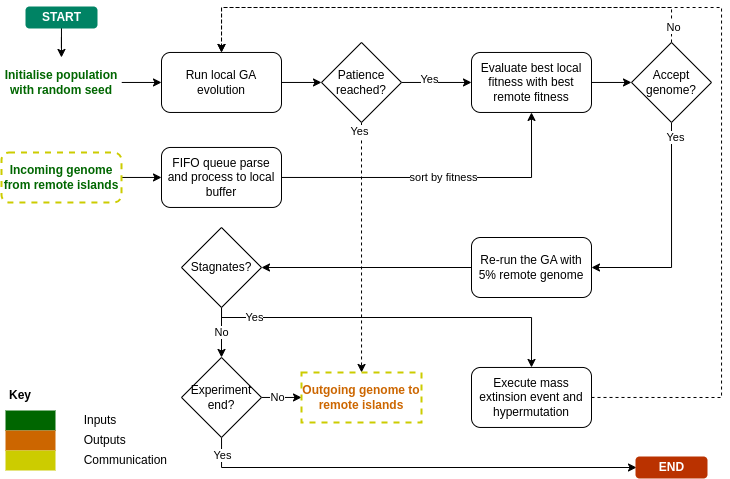
\includegraphics[width=0.65\textwidth]{ga.png}
    \caption{Island Model Flowchart}
    \label{fig:ga}
\end{figure*}

Our implementation employs an elitist migration strategy, this happens when the local GA reaches a patience threshold and the agent pushes its "best" (lowest fitness score) genome to other swarm members via ESP-NOW. The incoming remote genes from another peer are integrated into the local population by replacing the worst performing $5\%$ individuals, this value was chosen to preserve genomic high locally.\\ 

To avoid stagnation over a local-minimum, a mass extinction event together with a hyper-mutation mechanism tracks consecutive non-improving generations. Once a set of conditions is reached (Table X), the mutation probability is temporarily increased to escape local optima and lowest performing half of the population is re-initialised. This is done to promote exploration across the swarm and prevent premature convergence. 

\subsection{Real Time Operating System}

Each swarm member boots into a FreeRTOS runtime by calling \texttt{app\_main()}, which performs the initialisation of the following components: non-volatile storage, I2C peripherals, RTC, SD card, and ESP-NOW. Figure X illustrates the sequence of these and their relation to the tasks that are spawned during run time. Some of these tasks include:
\begin{itemize}
  \item \texttt{i2c\_task}: Handles communication with the I2C peripherals, including the AXP192 power supply, the IR board, the display and the Pololu 3pi+.
  \item \texttt{gui\_task}: Manages the UI on the M5Stack display, used for real-time feedback and debugging.
  \item \texttt{ota\_task} (conditional): Manages OTA updates if a new version is available in S3 (Section \ref{sec:ota}).
  \item \texttt{espnow\_task}: Manages ESP-NOW communication between swarm members, handles message sending and receiving.
  \item \texttt{ga\_task}: Runs the local GA and coordinates with other tasks to log and transmit data.
  \item \texttt{write\_task}: Handles SD card operations, including data logging and managing file storage.
\end{itemize} 

Inter-task coordination is managed by event groups and queues. The event groups are used to signal task completion and synchronise downstream operations, whereas queues are used to pass data between tasks that are operating in parallel. This enables multitasking and real-time processing of events, which differs from traditional SENSE, PLAN, ACT architectures that operate sequentially.\\

Following initialization and the conditional OTA update, each robot enters the experiment phase shown in Algorithm \ref{alg:swarm-loop}. Each robot is assigned a random starting point (seed) within the Rastrigin search space. The random seed is obtained via HTTPS from a server that streams quantum fluctuations in vacuum. This is to ensure that the seed is truly random and not influenced by any external factors. This initial population with its own set of random genes will thereafter undergo selection via a fitness function and genetic operators (mutation and crossover) to evolve the population.

The \texttt{ga\_task} evolves a local population until 30 generations are reached without achieving a 0.01 improvement in population fitness [REF]. At which point the best solution fitness score and genes are sent via ESPNOW to all swarm agents in a random order [NEED TO EXPLAIN WHY THIS WAS DONE]. ESPNOW send/receive callbacks measure per-packet latency (via ACKs), enqueue incoming frames to \texttt{ga\_buffer\_queue}, and count bytes for a throughput timer. The \texttt{espnow\_task} then dequeues and parses all events, updating statistics and evaluating remote genomes to \texttt{ga\_integrate\_remote\_solution}. 

An experiment is terminated when one of the following criteria is met:
\begin{enumerate}
  \item \textbf{Global Solution Achieved}: Any robot attains the exact global minimum of the Rastrigin function (fitness\,=\,0).
  \item \textbf{Time Limit Exceeded}: A configurable maximum duration (e.g., 10 minutes) elapses without global convergence.
\end{enumerate}
Upon termination, all ESPNOW tasks drain pending message queues, final fitness and communication metrics are written to the SD card, and log files are uploaded to an Amazon S3 bucket over HTTPS. Finally, the system de‐initializes peripherals (Wi‐Fi stopped, SD card unmounted, IR board halted) to ensure a clean shutdown.

\begin{algorithm*}[h]
\caption{Experimental Run Loop\label{alg:swarm-loop}}
\begin{algorithmic}[1]
  \State \textbf{Init} peripherals, Wi-Fi, ESPNOW, tasks, event groups, queues
  \State Fetch quantum seed via HTTPS; \Call{init\_ga}{seed}
  \Loop
    \State \textbf{Run GA:} \Call{evolve}{}
    \State Wait until \texttt{ga\_ended} \Comment{set in \texttt{ga\_complete\_callback}}
    \State \Call{espnow\_push\_best\_solution}{local\_best}
    \State $ga\_has\_run\_before \gets \mathrm{true}$; $s\_last\_ga\_time \gets \mathrm{now}$
    \State \Call{drain\_buffered\_messages}{} \Comment{Dequeue all ESPNOW frames}
    \ForAll{msg in \texttt{ga\_buffer\_queue}}
      \State \Call{ga\_integrate\_remote\_solution}{msg.genes}
    \EndFor
    \State \Call{check\_hyper\_mutation}{} \Comment{Adjust mutation if stagnated}
    \State Reset \texttt{ga\_ended}
  \EndLoop
\end{algorithmic}
\end{algorithm*}

\subsection{Communication Layer}

For our implementation of ESP-NOW, each swarm robot was pre-configured with the MAC addresses of all peers to facilitate direct communication. One key aspect to point out in this implementation is that connection handling and device pairing, which oversees how swarm members join and leave a connection. In its most basic form, we created a loop that goes over each MAC address and tries to rely a direct message to each other member in the swarm, to server as our benchmark. It is understood that the implications of this can have an impact on data loss and latency of the network. % add the event driven one-way communication
This communication protocol was designed to avoid having to handle pull type protocols which would involve having to handle requests and responses in a sequential manner.

Using the IR board, described previously. We connected the M5Stack via the external I2C port, furthermore we had to use the Arduino library as a component of the ESP-IDF implementation for the this to work, this was due to compatibility issues between ESP-IDF and Arduino libraries. The board itself is running with an Arduino Nano to process the IR signals into messages and then sending this data accross via the SDA/SCL pins. One major implication for this, was the need to change the FreeRTOS clock speed from 100Hz to 1000Hz which improves responsiveness but at the cost of higher CPU load and power consumption. Some key parameters also include the frequency if the I2C itself which was set at 100kHtz and the master/slave configuration (M5 being the master device), this is initialized from the M5 once powered on after the 5V bus is switched on (to power the board). For more details regarding the IR board implementation please see X. 


We used ESPNOW by pre-registering each swarm member’s MAC address, enabling unicast communication once the local GA finishes. Incoming data is placed on a queue for processing, and latency is measured via ACK callbacks. A periodic timer tracks overall throughput, logging key events as data arrives. This setup ensures efficient message handling without interfering with ongoing local genetic algorithm as it run co-curretly.

\subsubsection{Topology Inference}

Based on the baseline results, we propose to investigate the impact of different communication schemes on the emergent swarm topology by introducing two message sending strategies: \textbf{RANDOM} and \textbf{COMM\_AWARE}. From version 0.4 onwards, these schemes are implemented in the communication layer and are designed to influence the order and priority with which each agent sends its best solution to its peers. The aim is to understand how these strategies affect the connectivity and robustness of the swarm network.\\

The expectation is that both \textbf{RANDOM} and \textbf{COMM\_AWARE} will result in a fully connected network over time, as each agent attempts to send messages to all other agents. However, the \textbf{COMM\_AWARE} scheme is designed to preferentially strengthen links with agents that are either furthest away (as inferred by higher latency and lower RSSI) or have not yet established a reliable connection (null metrics). This should result in a network where communication is dynamically biased towards improving weak or unmeasured links, using latency and RSSI as psuedo-metrics for distance allows the swarm to adapt to the percieved communication quality without having to know the exact positition of each member relative to itself. This is particularly useful in scenarios where the deployment is remote or there is no infrastructure available to track position.\\

The two communication schemes are implemented as follows:

\begin{itemize}
    \item \textbf{RANDOM}: Each agent shuffles the list of peer MAC addresses using a Fisher-Yates shuffle (with a random seed) before sending its message. This ensures that the order of communication is random for each broadcast cycle, preventing bottlenecks or biases.
    \item \textbf{COMM\_AWARE}: Each agent ranks its peers based on the most recent measurements of communication quality, specifically the last known latency (measured via ACK round-trip time) and RSSI (received signal strength indicator). Peers with unknown metrics (null latency or RSSI) are prioritized first to ensure all links are measured. Among the rest, peers are scored by normalizing both latency and RSSI, and those with the worst (highest latency, lowest RSSI) are prioritized for message sending.
\end{itemize}

The following pseudocode outlines the logic for each scheme:

\paragraph{RANDOM Communication Scheme}
\begin{algorithm}[H]
\caption{Randomized Peer Selection}
\begin{algorithmic}[1]
\State \textbf{Input:} List of peer MAC addresses
\State Shuffle the list using Fisher-Yates and a random seed
\For{each peer in shuffled list}
    \If{peer is not self}
        \State Send message to peer
    \EndIf
\EndFor
\end{algorithmic}
\end{algorithm}

%TODO: UPDATE THIS TO MENTION 50% SCOPE OF NETWORK
\paragraph{COMM\_AWARE Communication Scheme}
\begin{algorithm}[H]
\caption{Communication-Aware Peer Ranking}
\begin{algorithmic}[1]
\State \textbf{Input:} List of peer MAC addresses, last known RSSI and latency for each peer
\For{each peer}
    \If{RSSI or latency is null}
        \State Assign highest priority
    \Else
        \State Normalize RSSI and latency across all peers
        \State Compute score: $score = norm\_latency + norm\_rssi$
    \EndIf
\EndFor
\State Sort peers: null metrics first, then by descending score (worst first)
\For{each peer in sorted list}
    \If{peer is not self}
        \State Send message to peer
    \EndIf
\EndFor
\end{algorithmic}
\end{algorithm}

These communication schemes are only meaningful in swarms with more than two robots, as the benefits of dynamic peer selection and ranking emerge only in larger networks. Furthermore, this approach is specifically designed for \textbf{UNICAST} communication, where messages are sent directly to individual peers and round-trip latency can be measured via ACKS. In the case of \textbf{BROADCAST} communication, it is not practical to measure per-peer latency, although RSSI can still be estimated by the receiver for each incoming message.
%need to decide if we will test broadcast....

\subsubsection{Limited-Rate Communication (TOKEN\_BUCKET)}

Inspired by the “less-is-more” (LIME) effect reported for Kilobots using infrared links \cite{aust_hidden_2022}, we add a *token-bucket* limiter to the ESP-NOW layer and treat its quota as an **independent variable**.  
Each agent is given a small budget of $1$ message in a sliding window of length $10000$ milliseconds.  When the bucket is empty the agent must keep silent until the window refreshes, regardless of how often its GA stagnates or improves.  This caps the *total* interaction rate per robot rather than merely spacing individual transmissions, closely matching the physical connectivity ceiling studied in \cite{aust_hidden_2022} but now in a 2.4-GHz ESPNOW setting.

\paragraph{Parameters}
\begin{itemize}
  \item $B$ – message budget (tokens) per window
  \item $W$ – window length in milliseconds
  \item $t_{\mathrm{last}}$ – start-time of current window (initialised at boot)
  \item $\mathit{tokens}$ – remaining tokens in the current window
\end{itemize}

\begin{algorithm}[H]
\caption{Token-Bucket Throttled Send}
\label{alg:token_bucket}
\begin{algorithmic}[1]
\State \textbf{procedure} \textsc{MaybeSend}$(\mathit{payload})$
\State $now \gets$ \Call{CurrentTimeMs}{}
\If{$now - t_{\mathrm{last}} \ge W$}               \Comment{window refresh}
    \State $\mathit{tokens} \gets B$
    \State $t_{\mathrm{last}} \gets now$
\EndIf
\If{$\mathit{tokens} = 0$}
    \State \textbf{return}   \Comment{bucket empty $\rightarrow$ no send}
\EndIf
\If{\Call{ImprovedFitness}{}}
    \State $\mathit{tokens} \gets \mathit{tokens} - 1$
    \State \Call{ESP\_NOW\_Send}{$\mathit{payload}$}
\EndIf
\end{algorithmic}
\end{algorithm}

By tightening $B$ (or enlarging $W$) we progressively restrict social signalling. Following the findings in \cite{aust2022hidden}, we hypothesise that:

\begin{enumerate}
  \item \textbf{Convergence speed will decrease}: fewer migrations mean each island explores locally for longer before external influence arrives.
  \item \textbf{Task performance will improve}: reduced network contention and wider behavioural diversity should help the swarm escape local minima, yielding lower global Rastrigin scores by the termination time.
\end{enumerate}

Thus, the experiment sweeps $B\in\{1,2,4,8\}$ (with $W=10\,\mathrm{s}$) to test whether the LIME phenomenon extends from low-bandwidth IR to high-bandwidth ESPNOW links.


\newpage
\section{Preliminary Sensitivity Analysis}

\begin{figure*}[h]
    \centering
    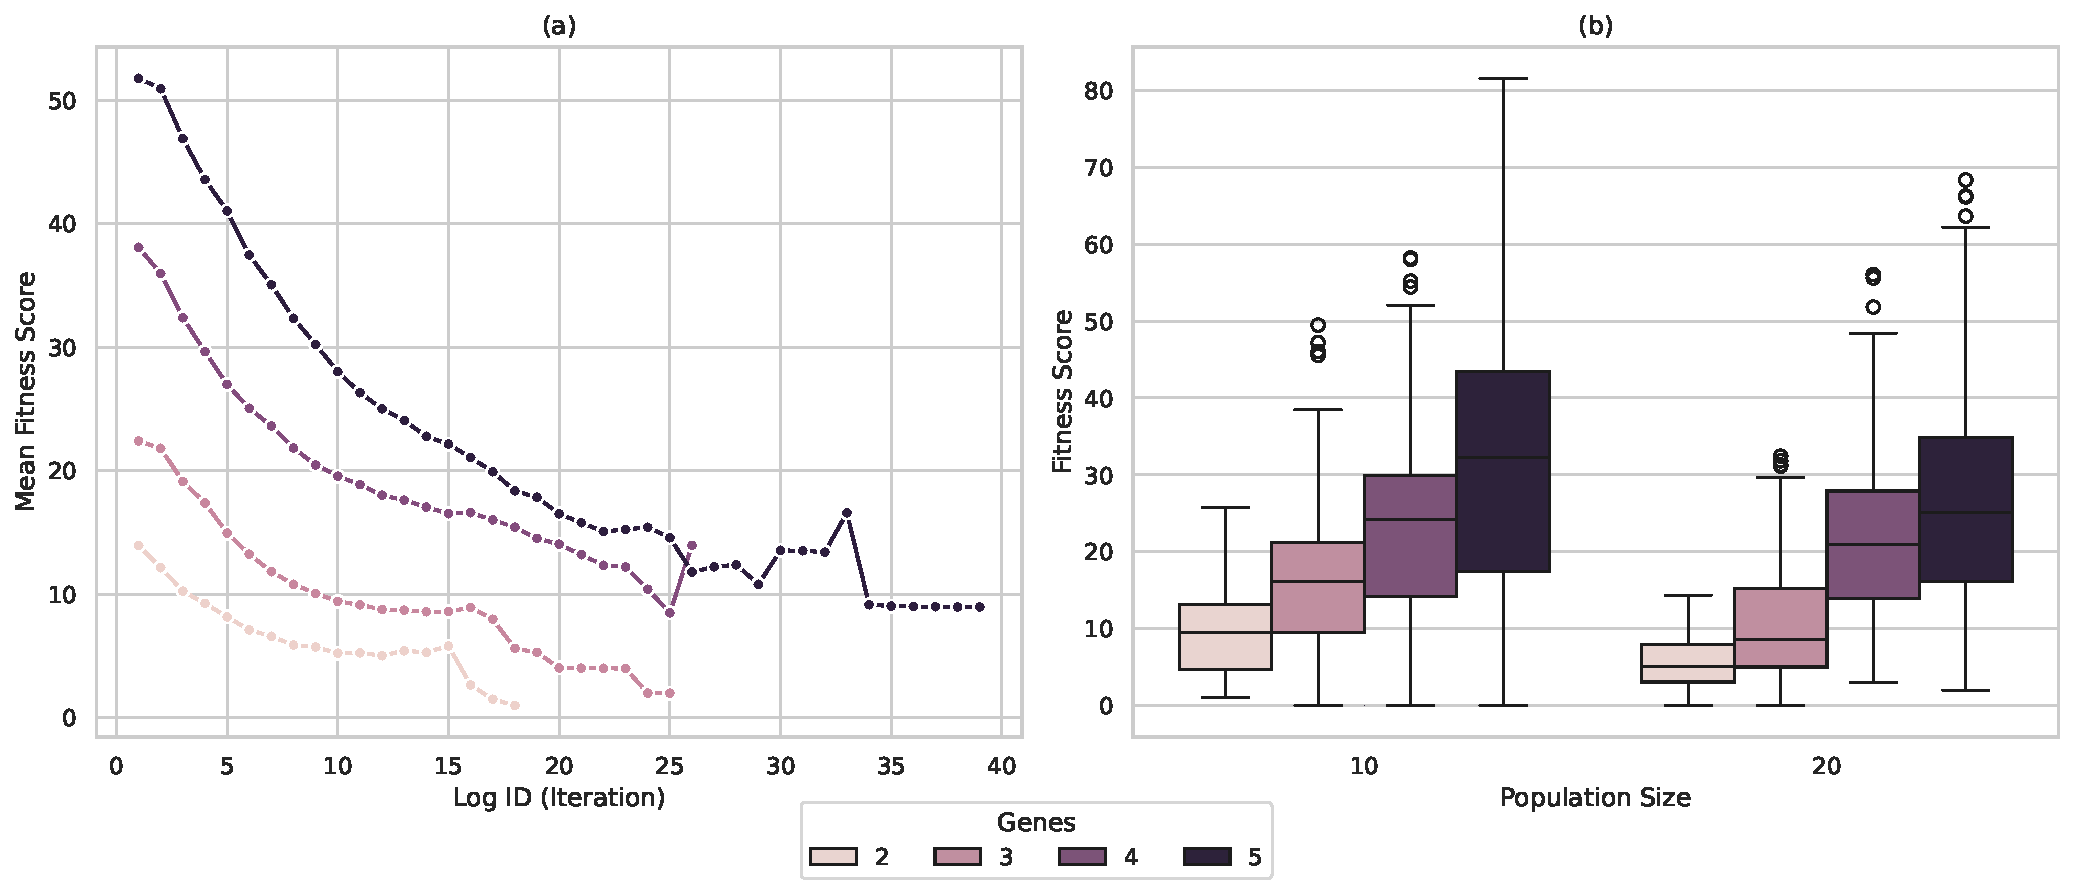
\includegraphics[width=1\textwidth]{ga_prelim_analysis.pdf}
    \caption{a: Number of iterations for algorithm to converge to either a global or local minimum. b: Fitness distribution by population size and genes.}
    \label{fig:ga_prelim_analysis}
\end{figure*}

Using a single robot, a preliminary analysis was conducted to identify suitable parameters for solving the Rastrigin function under varying population sizes (10, 20) and gene dimensions (2, 3, 4, 5). A total of \textbf{136 experiments} were performed, each terminating if fitness failed to improve beyond a \textbf{0.001 threshold} over \textbf{20 consecutive epochs} (patience). %TODO: Include reference for the patience parameter
If the global optimum (fitness=0) was not reached, the run was considered to have converged into a local minimum. Across all runs, the time taken to converge ranged \textbf{between 0 to 3 seconds}, reflecting the early stopping triggered by the patience setting. As shown in Figure~\ref{fig:ga_prelim_analysis}, larger populations and higher iteration counts generally yielded lower final fitness, consistent with the genetic algorithm’s search properties.\\

%include table of parameters kept constant for GA. And all other config parameters that were kept constant.

A practical takeaway from the data is that using five genes is sufficiently challenging to extend the runtime into the range of minutes rather than seconds, even though a single robot with fewer genes can solve the function in only a couple of seconds. This configuration will ensure that experiments in a swarm environment will involve cooperation, where the exchange of best solutions between members could enable global convergence for a five-dimensional Rastrigin function.

\newpage
\section{Base Line Results}

\begin{figure*}[t]
  \centering
  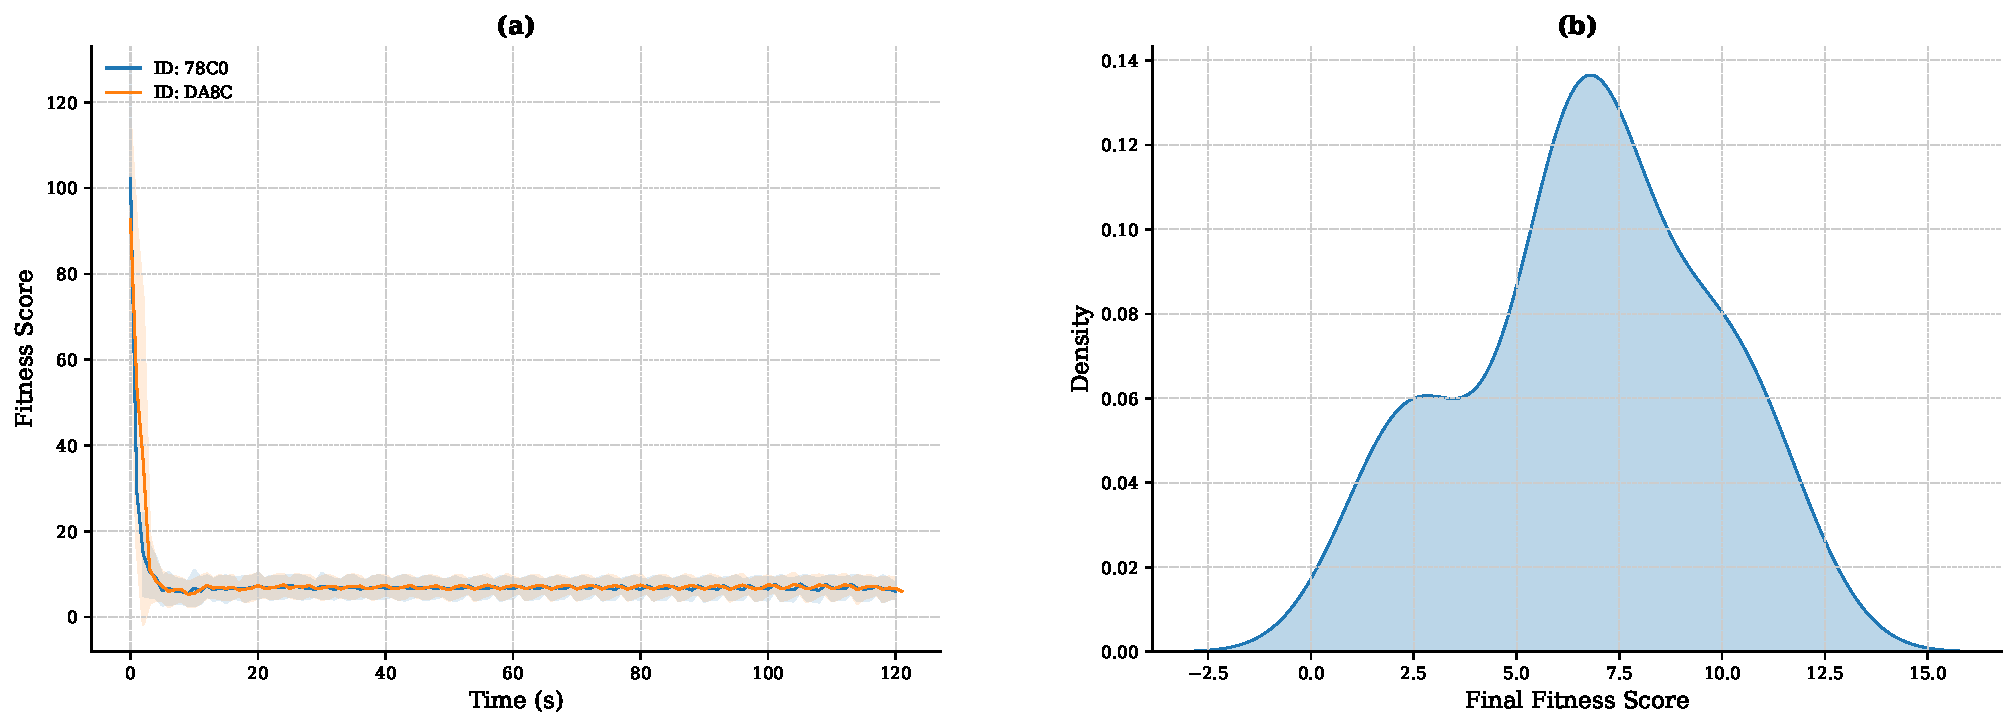
\includegraphics[width=1\textwidth]{base_fitness_stats.pdf}
  \caption{a: Mean population fitness score for each agent over time,  b: Final fitness score density distribution, c: Mean CPU utilisation over time.}
  \label{fig:base_fitness_stats}
\end{figure*}

Figure \ref{fig:base_fitness_stats} shows the fitness scores and system metrics for a deployment of two agents. A total of 34 experimens were conducted, out of which 6 experiments had to be excluded from the analysis as the data did not reach the S3 for at least one of the devices, mainly due to a bug in the code that was caused by the messages arriving late and the system not being able to handle these in the de-initiasation sequence. This bug was addressed since version 0.4 of the project, which allows the \texttt{espnow\_task} to drain the queue for any late messages coming in.\\

\begin{table}[h]
  \centering
  \caption{Baseline Configuration Parameters}
  \label{tab:base_config}
  \begin{tabular}{l@{~=~}l}
    app\_ver & 0.3\\
    data\_link & ESPNOW\\
    routing & unicast\\
    population\_size & 30\\
    max\_genes & 5\\
    patience & 30\\
    migration\_type & asynchronous\\
    migration\_scheme & elitist\\
    migration\_rate & 1\\
    migration\_frequency & patience based\\
    hyper\_mutation & true\\
    mass\_extinction & true\\
    robot\_speed & 0\\
    topology & fully connected\\
    experiment\_time & 120 s\\
  \end{tabular}
\end{table}

Using the baseline parameters shown in Table \ref{tab:base_config}, we can see that none of the experiments was able to reach the global minimun of 0.0 in terms of the fitness score. The mean final fitness score achieved was X.X indicating that a local minimum is reached, whereas the rate of the converge takes place within the first 10 seconds of the experiment and stagnates thereafter. This behaviour is aligns with a large CPU utilisation in both cores at the start of the experiment, from observations this can be attributed to the first local GA running in each agent which then stagnates after exchanging a few messages with the other peer. Taking this into consideration, for experiments from version 0.4 onwards the population size and number of genes are doubled to 60 and 10 respectively, to ensure diversity in the gene pool with the trade off of slower convergence.\\

\begin{figure*}[b]
  \centering
  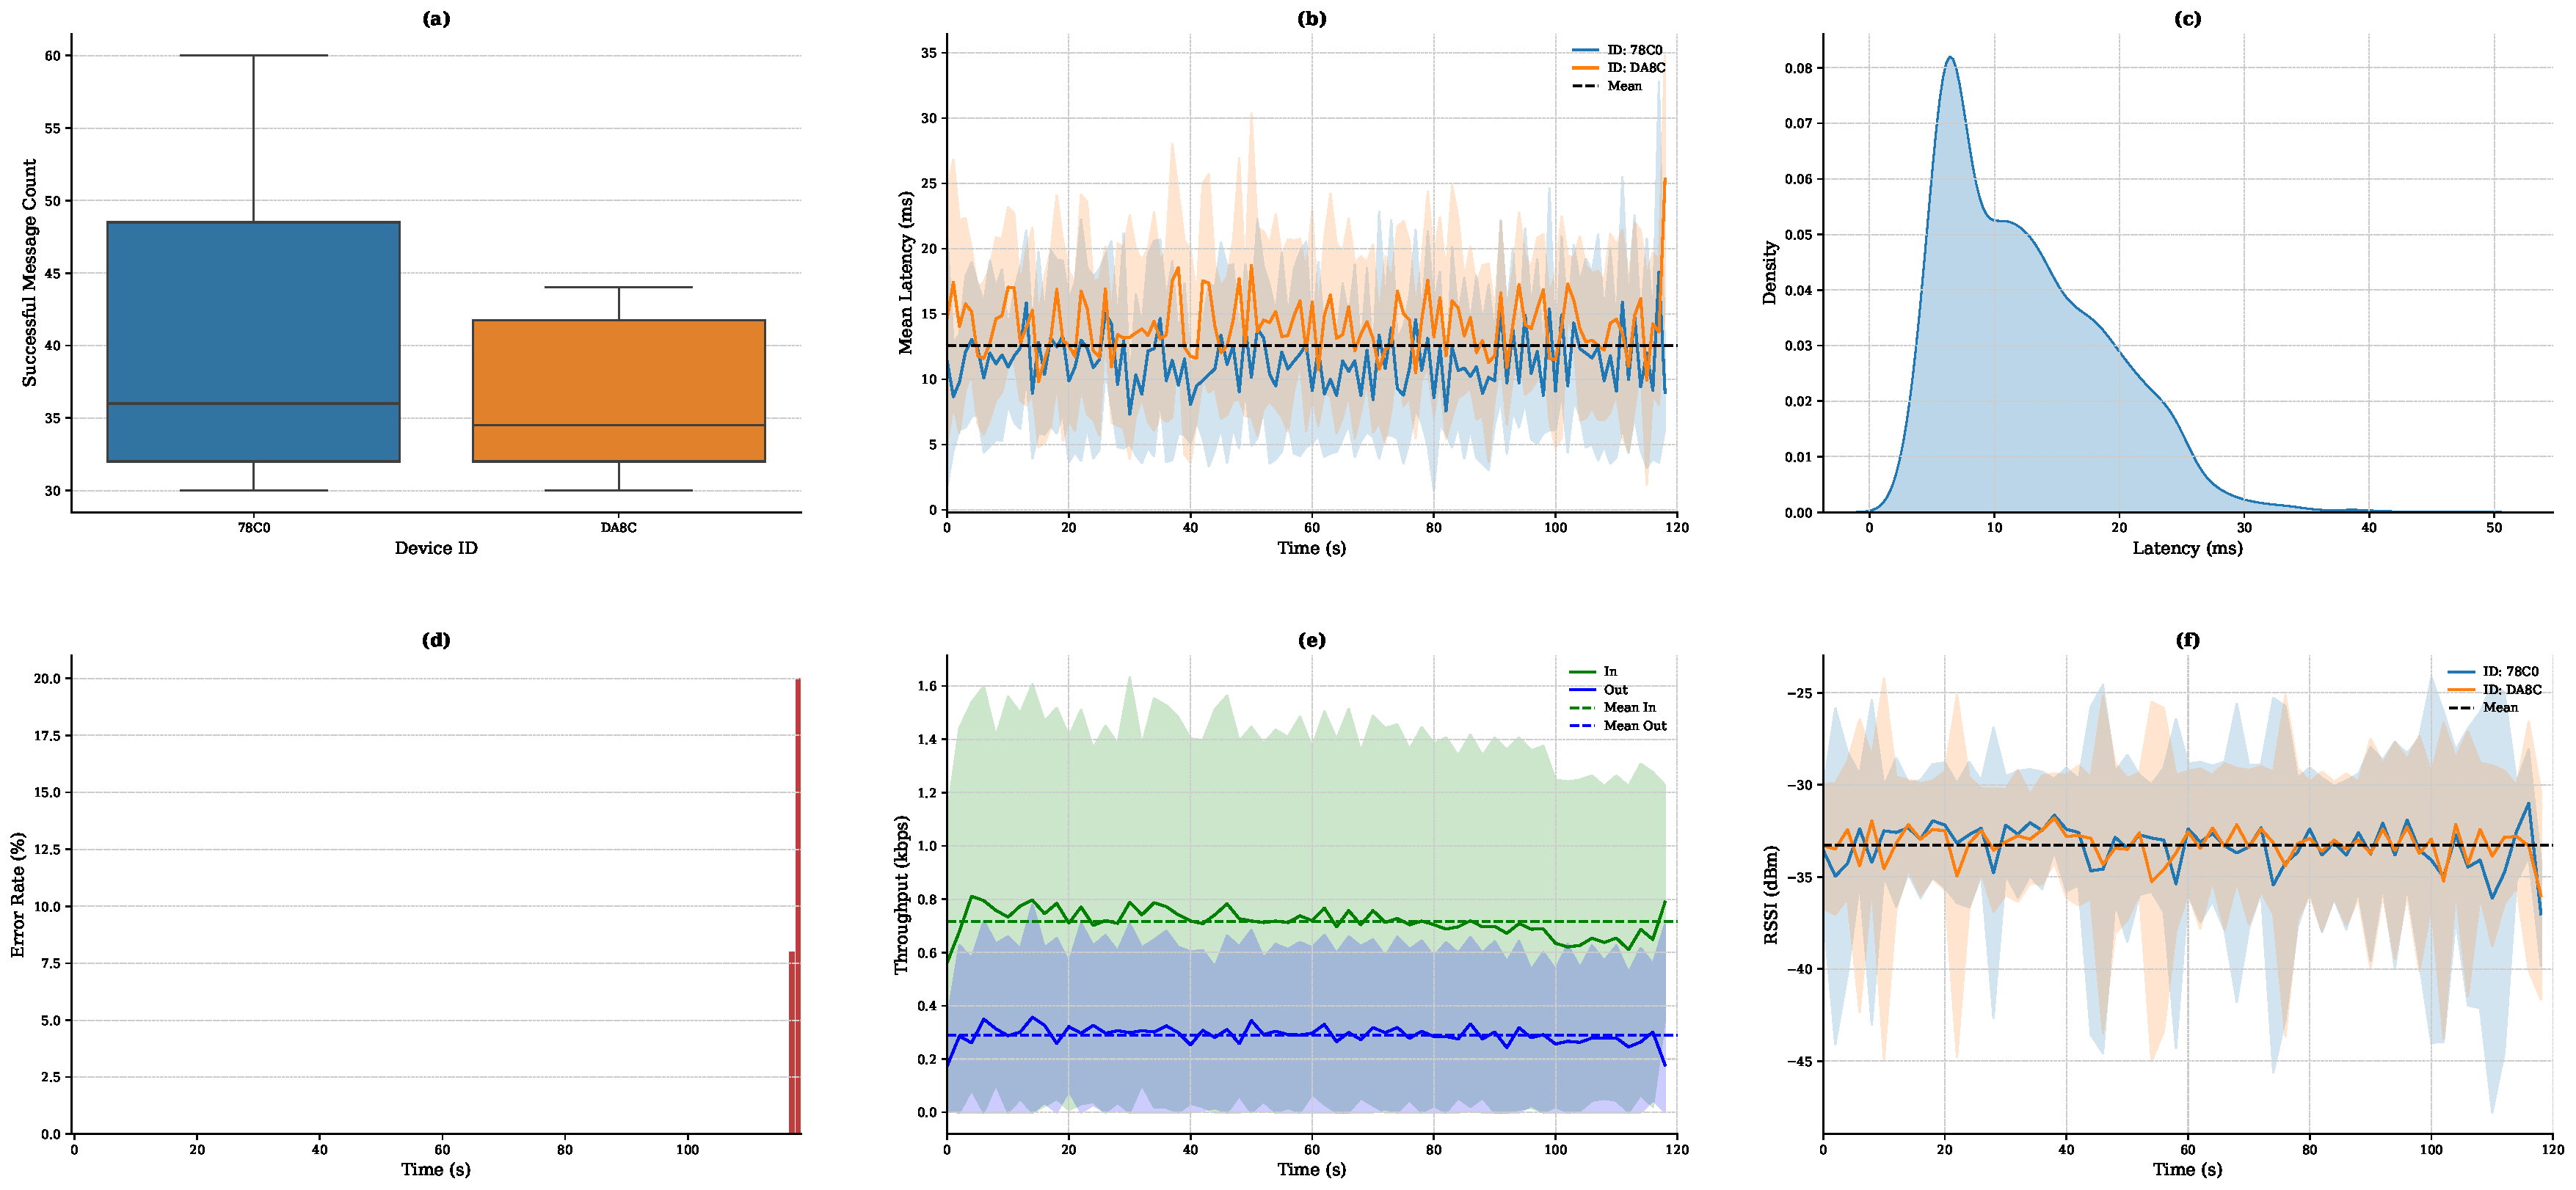
\includegraphics[width=1\textwidth]{base_comm_stats.pdf}
  \caption{a: Message sent distribution by each device,  b: Mean latency by device over time, c: Latency distribution accross all experiments, d: Mean error rate from failed messages over time, e: Mean throughput In/Out over time, f: Mean RSSI by device over time.}
  \label{fig:base_comm_stats}
\end{figure*}

Figure \ref{fig:base_comm_stats} shows the communication statistics for the same deployment of the two agents and the top level metrics are described in Table X. The mean latency was X.X ms, with a maximum latency of X.X ms. The latency statistics show that the ESPNOW protocol is able to handle the communication between the agents with low latency which is in line with other IoT applications REF. One artifact of the data worth noting is that high latencies were observed at the end of the experiments where the error rate was the highest, this is likely due to the longer delay in recieving an ACK from the other peer which has already de-initialised the ESPNOW task and is no longer able to respond to the messages. This would indicate that larger latencies are driven by failed messages pending an ACK. Note that in our base config we set the ESPNOW parameter \texttt{ESPNOW\_MAX\_RETRIES} to 0, which means that the messages are not retried if they fail to be sent. This is done to avoid having to handle pull type protocols which would involve having to handle requests and responses in a sequential manner.\\

\begin{table}[h]
  \centering
  \caption{Baseline Network Performance Metrics}
  \label{tab:baseline_network_metrics}
  \begin{tabular}{ll}
  \toprule
  \textbf{Metric} & \textbf{Value} \\
  \midrule
  Network Jitter (ms)      & 8.80  \\
  Max Bandwidth (kbps)     & 1.41  \\
  Network Error Rate (\%)  & 0.01  \\
  QoS (0--1)               & 0.7   \\
  \bottomrule
  \end{tabular}
\end{table}

The mean In/Out throughput achieved was X.X kbps and X.X respectively. It is worth noting that the higher In throughput suggests that there is an imbalance in the number of messages being exchanged, this can be confirmed by plot (a) in Figure \ref{fig:base_comm_stats} that shows one agent sending more messages than the other. This is likely due to the fact that the agents are not perfectly synchronised by the RTC, this means they finalise their first local GA at different times (also impacted by the random seed). This means that one agent is able to send its best solution before the other agent has a chance to send its own, this is an artifact of the current implementation and might have to be addressed in future work. Note that the expectation is that the network throughput will increase as the swarm increases in size, where the theoretical max throughput for ESPNOW is 214 kbps by device.\\ 

The mean RSSI accross all devices was X.X dBm, which in in a range that indicates that the communication link is stable and reliable REF. It is worth noting that the RSSI is measured between peers and therefore it can be used as an indicative measure of the distance between agents though we also expect that the RSSI will be affected by the environment and obstacles in between the agents. This influence will be explored in Section X where the topology of the swarm is varied to see how this affects the communication performance.\\



% Add more chapters as needed

\newpage
\printbibliography

\end{document}